\hypertarget{index_pageTOC}{}\subsection{Content}\label{index_pageTOC}

\begin{DoxyEnumerate}
\item \hyperlink{index_Introduction}{Introduction}
\begin{DoxyEnumerate}
\item \hyperlink{index_Module_Intro}{Module}
\item \hyperlink{index_Project_Intro}{Project}
\end{DoxyEnumerate}
\item \hyperlink{index_ceusapi}{C\+E\+U\+S A\+P\+I}
\begin{DoxyEnumerate}
\item \hyperlink{index_auth}{auth.\+php}
\item \hyperlink{index_list}{list.\+php}
\item \hyperlink{index_curr}{curr.\+php}
\item \hyperlink{index_detail}{detail.\+php}
\item \hyperlink{index_Errors}{Errors}
\end{DoxyEnumerate}
\item \hyperlink{index_Modules}{Modules}
\begin{DoxyEnumerate}
\item \hyperlink{index_CEUS2Drupal}{C\+E\+U\+S2\+Drupal}
\begin{DoxyEnumerate}
\item \hyperlink{index_Import}{Import}
\item \hyperlink{index_change_management}{Change Management}
\end{DoxyEnumerate}
\item \hyperlink{index_Drupal2ITSV}{Drupal2\+I\+T\+S\+V}
\item \hyperlink{index_Drupal2PDF}{Drupal2\+P\+D\+F}
\item \hyperlink{index_Drupal2AGG}{Drupal2\+A\+G\+G}
\begin{DoxyEnumerate}
\item \hyperlink{index_json}{Drupal J\+S\+O\+N Interface}
\item \hyperlink{index_plugin}{C\+K\+Editor Plug-\/in}
\item \hyperlink{index_graph}{Graph.\+js}
\end{DoxyEnumerate}
\item \hyperlink{index_Other}{Other}
\end{DoxyEnumerate}
\item \hyperlink{index_Development}{Development}
\begin{DoxyEnumerate}
\item \hyperlink{index_Authors}{Authors}
\item \hyperlink{index_versionnumbers}{Version Numbers}
\item \hyperlink{index_versioncontrol}{Version Control}
\end{DoxyEnumerate}
\item \hyperlink{index_Included}{Included Libraries/\+Files}
\end{DoxyEnumerate}\hypertarget{index_Introduction}{}\subsection{Introduction}\label{index_Introduction}
\hypertarget{index_Module_Intro}{}\subsubsection{Module}\label{index_Module_Intro}
This documentation describes the custom module \char`\"{}stukowin\char`\"{} for \href{http://drupal.org/}{\tt Drupal}. Drupal is a free and widely-\/used content management system (C\+M\+S), which provides the possibility to extend it by implementing proprietary modules that hook into the Drupal core system. The basic idea of this module is to connect the Drupal system with the curricula development and support system (C\+E\+U\+S) provided by the \href{http://jku.at}{\tt Johannes Kepler University in Linz}, available at \href{https://lss.jku.at/wiki/index.php/Main/CEUS}{\tt https\+://lss.\+jku.\+at/wiki/index.\+php/\+Main/\+C\+E\+U\+S} and \href{https://lss.jku.at/studienhandbuch/}{\tt https\+://lss.\+jku.\+at/studienhandbuch/}. The main goal of this method was to reduce the maintenance effort needed for keeping the curricula data on a website up to date.

The module is composed of four components, as seen \hyperlink{index_Modules}{below}, each of which provides different functionalities to reduce the administrative effort and all of which are somehow interconnected.\hypertarget{index_Project_Intro}{}\subsubsection{Project}\label{index_Project_Intro}
This module was created as a result of the course \char`\"{}\+I\+T Project\char`\"{}, a part of the bachelor's degree in business informatics at J\+K\+U, during the summer semester 2014.

The project name is \char`\"{}\+Relaunch der Homepage der Studienkommission W\+I\+N\char`\"{}. The original site can be found at \href{http://stukowin.jku.at/}{\tt http\+://stukowin.\+jku.\+at/}. The project sponsor is Dr. Stefan Berger (\href{mailto:stefan.berger@jku.at}{\tt stefan.\+berger@jku.\+at}).

The main functional project requirements include the following\+:
\begin{DoxyEnumerate}
\item Automatic import of curricula data from C\+E\+U\+S
\item Possibility of editing curricula entries after the import
\item Version management for curricula entries
\item Automatically displaying different curricula on the site
\item Possibility to create new ideal courses of studies (\char`\"{}\+Idealtypischer Studienverlauf\char`\"{}, I\+T\+S\+V) and specialisation curricula
\item Archiving and exporting curricula in the form of P\+D\+F documents
\end{DoxyEnumerate}

\begin{DoxyRemark}{Remarks}
This documentation is one of four documents that make up the entire project documentation, namely the operator guide, the user guide and the test documentation.
\end{DoxyRemark}
\hypertarget{index_ceusapi}{}\subsection{C\+E\+U\+S A\+P\+I}\label{index_ceusapi}
In order to make functional requirements such as displaying curricula and course details possible, it is necessary to extract the required data from C\+E\+U\+S. For this reason, J\+K\+U offers a J\+S\+O\+N A\+P\+I for C\+E\+U\+S at \href{https://lss.jku.at/studienhandbuch/api/0.1}{\tt https\+://lss.\+jku.\+at/studienhandbuch/api/0.\+1} (Note that this U\+R\+L is not available without authentication credentials). This A\+P\+I was developed for this project (hence the version number of {\itshape 0.\+1}) and is still prone to changes. Due to its novelty, no documentation for the A\+P\+I exists, which is why we try our best to document it together with our own module documentation. \begin{DoxyNote}{Note}
This is not the official documentation of the C\+E\+U\+S A\+P\+I, it is merely based on our own knowledge about it. 

For any questions concerning the A\+P\+I please contact Andreas Roesch (\href{mailto:Andreas.Roesch@jku.at}{\tt Andreas.\+Roesch@jku.\+at}) or Mag. Martin Stabauer (\href{mailto:martin.stabauer@jku.at}{\tt martin.\+stabauer@jku.\+at})
\end{DoxyNote}
This A\+P\+I provides four public methods which will be described below.\hypertarget{index_auth}{}\subsubsection{auth.\+php}\label{index_auth}
\begin{TabularC}{2}
\hline
\rowcolor{lightgray}{\bf Method }&{\bf /auth.php  }\\\cline{1-2}
Input &\char`\"{}username\char`\"{},\char`\"{}password\char`\"{} \\\cline{1-2}
Output &\char`\"{}authtoken\char`\"{} \\\cline{1-2}
\end{TabularC}
The method {\ttfamily auth} serves the purpose of authenticating a user and returns a token which is required for every other A\+P\+I method call. The user credentials at the time of development are as follows\+: \begin{DoxyVerb}User: dke2
Password: studke2hb
\end{DoxyVerb}
\hypertarget{index_list}{}\subsubsection{list.\+php}\label{index_list}
\begin{TabularC}{2}
\hline
\rowcolor{lightgray}{\bf Method }&{\bf /list.php  }\\\cline{1-2}
Input &\char`\"{}authtoken\char`\"{} \\\cline{1-2}
Output &Array of Branch objects (see below) in J\+S\+O\+N \\\cline{1-2}
\end{TabularC}


The method {\ttfamily list} returns an array of all curricula to which the user has access. In the scope of this project, these are the bachelor and master studies in business informatics. The curricula are returned in the data structure shown below\+:


\begin{DoxyImage}
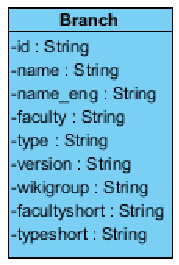
\includegraphics{Branch}
\caption{Branch Objects}
\end{DoxyImage}
 The data structure contains a few elements. For this project, only the following are relevant\+:

\begin{TabularC}{2}
\hline
\rowcolor{lightgray}{\bf Field }&{\bf Description  }\\\cline{1-2}
id &C\+E\+U\+S id of the curriculum. This id is needed for the \hyperlink{index_curr}{curr.php} method. \\\cline{1-2}
name &German name of the curriculum \\\cline{1-2}
namme\+\_\+en &English name of the curriculum \\\cline{1-2}
faculty &Faculty of the curriculum \\\cline{1-2}
type &Bachelor or master studies \\\cline{1-2}
typeshort &Short version of the type ({\itshape B} or {\itshape M}) \\\cline{1-2}
version &Semester when the curriculum was introduced (e.\+g. {\itshape 2013\+W}) \\\cline{1-2}
\end{TabularC}
\hypertarget{index_curr}{}\subsubsection{curr.\+php}\label{index_curr}
\begin{TabularC}{2}
\hline
\rowcolor{lightgray}{\bf Method }&{\bf /curr.php  }\\\cline{1-2}
Input &\char`\"{}authtoken\char`\"{}, \char`\"{}id\char`\"{} \\\cline{1-2}
Output &Object of type curriculum (see below) in J\+S\+O\+N \\\cline{1-2}
\end{TabularC}
The method {\ttfamily curr} returns general information about a curriculum and, more importantly, its structure. A curriculum is identified throug the {\itshape id} returned by \hyperlink{index_list}{list.php} method. Curricula are returned in the following structure\+:


\begin{DoxyImage}
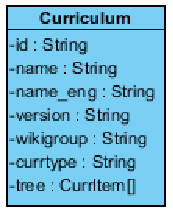
\includegraphics{Curriculum}
\caption{Curriculum Objects}
\end{DoxyImage}
 All but the last element have already been described in \hyperlink{index_list}{list.php} The last one is described below\+:

\begin{TabularC}{2}
\hline
\rowcolor{lightgray}{\bf Field }&{\bf Description  }\\\cline{1-2}
tree &A nested array of {\ttfamily Curr\+Items}, which represents the curriculum structure. The field {\ttfamily id} of each {\ttfamily Curr\+Item} is needed for the \hyperlink{index_detail}{detail.php} method. The field {\ttfamily subtree} contains the subcourses of each course \\\cline{1-2}
\end{TabularC}

\begin{DoxyImage}
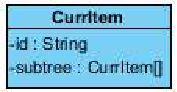
\includegraphics{CurrItem}
\caption{Curr\+Item Objects}
\end{DoxyImage}
 \hypertarget{index_detail}{}\subsubsection{detail.\+php}\label{index_detail}
\begin{TabularC}{2}
\hline
\rowcolor{lightgray}{\bf Method }&{\bf /detail.php  }\\\cline{1-2}
Input &\char`\"{}authtoken\char`\"{}, \char`\"{}id\char`\"{} \mbox{[},\char`\"{}lang\char`\"{}\mbox{]} \\\cline{1-2}
Output &Array of Detail objects (see below) in J\+S\+O\+N \\\cline{1-2}
\end{TabularC}
The method {\ttfamily detail} returns the details for one {\ttfamily Curr\+Item}. A {\ttfamily Curr\+Item} can be a subject (Fach), a module (Modul) or a simple course (Lehrveranstaltung). For localised data the optional parameter {\ttfamily lang} with the value \char`\"{}de\char`\"{} (German) or \char`\"{}en\char`\"{} (English) can be given. Details are returned in the folling data structure\+:


\begin{DoxyImage}
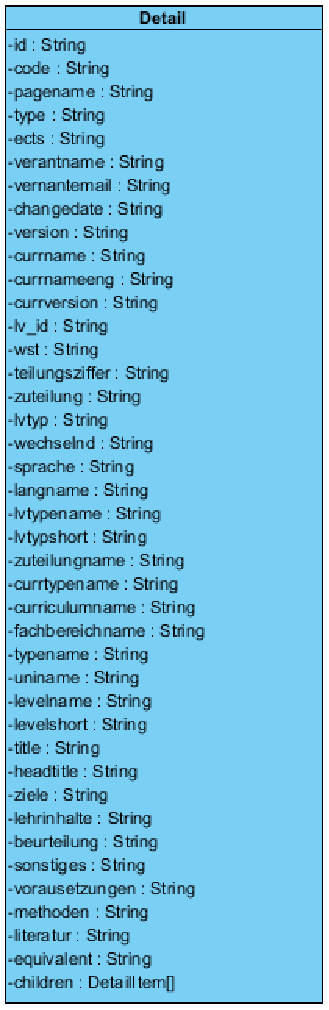
\includegraphics{Detail}
\caption{Detail Objects}
\end{DoxyImage}
 For this project, mainly the following elements are relevant\+:

\begin{TabularC}{2}
\hline
\rowcolor{lightgray}{\bf Field }&{\bf Description  }\\\cline{1-2}
ects &Credits for the course \\\cline{1-2}
verantname &Name of the person responsible for this course \\\cline{1-2}
verantemail &Email of the person responsible for this course \\\cline{1-2}
changedate &Date and time of the last change of this entry (in the format \char`\"{}\+Y\+Y\+Y\+Y-\/\+M\+M-\/\+D\+D hh\+:mm\+:ss\char`\"{}) \\\cline{1-2}
currname &Name of the curriculum that contains this course \\\cline{1-2}
wst &Semester periods per week (Semesterwochenstunden) for this course \\\cline{1-2}
langname &Language the course is held in \\\cline{1-2}
lvtypshort &Short type of the course (e.\+g. V\+L, U\+E, K\+V etc.) \\\cline{1-2}
lvatype &Long type of the course (Vorlesung, Uebung etc.) \\\cline{1-2}
typename &Long type of the entry (subject, module or course) \\\cline{1-2}
type &Number representative of the type of entry (1=subject, 2=module and 3=course) \\\cline{1-2}
title &Course title \\\cline{1-2}
ziele &Course goals \\\cline{1-2}
lehrinhalte &Contents of teaching \\\cline{1-2}
voraussetzungen &Course requirements \\\cline{1-2}
methoden &Teaching methods \\\cline{1-2}
\end{TabularC}
\hypertarget{index_Errors}{}\subsubsection{Errors}\label{index_Errors}
In case of an error, the C\+E\+U\+S A\+P\+I returns a J\+S\+O\+N object with the error message contained in the {\ttfamily error} field. Known errors are\+:
\begin{DoxyItemize}
\item Invalid id given
\item Missing parameter
\item Missing authentication token
\end{DoxyItemize}\hypertarget{index_Modules}{}\subsection{Modules}\label{index_Modules}
\hypertarget{index_CEUS2Drupal}{}\subsubsection{C\+E\+U\+S2\+Drupal}\label{index_CEUS2Drupal}
\hypertarget{index_Import}{}\paragraph{Import}\label{index_Import}
The import of data from C\+E\+U\+S to the Drupal environment is implemented in this component. All its functionality is collected in the \hyperlink{index_CEUS2Drupal}{C\+E\+U\+S2\+Drupal} component. The data model for the Drupal-\/internal representation of courses is defined in the module's \hyperlink{stukowin_8install}{install component}, the necessary database tables are automatically created during the installation. Because the A\+P\+I U\+R\+L and user credentials are prone to change, they need to be configurable. This is achieved in the \hyperlink{group___stukowin___module_ga55d453d5b6f8ae4e643308d8814e67a5}{admin menu}\+:


\begin{DoxyImage}
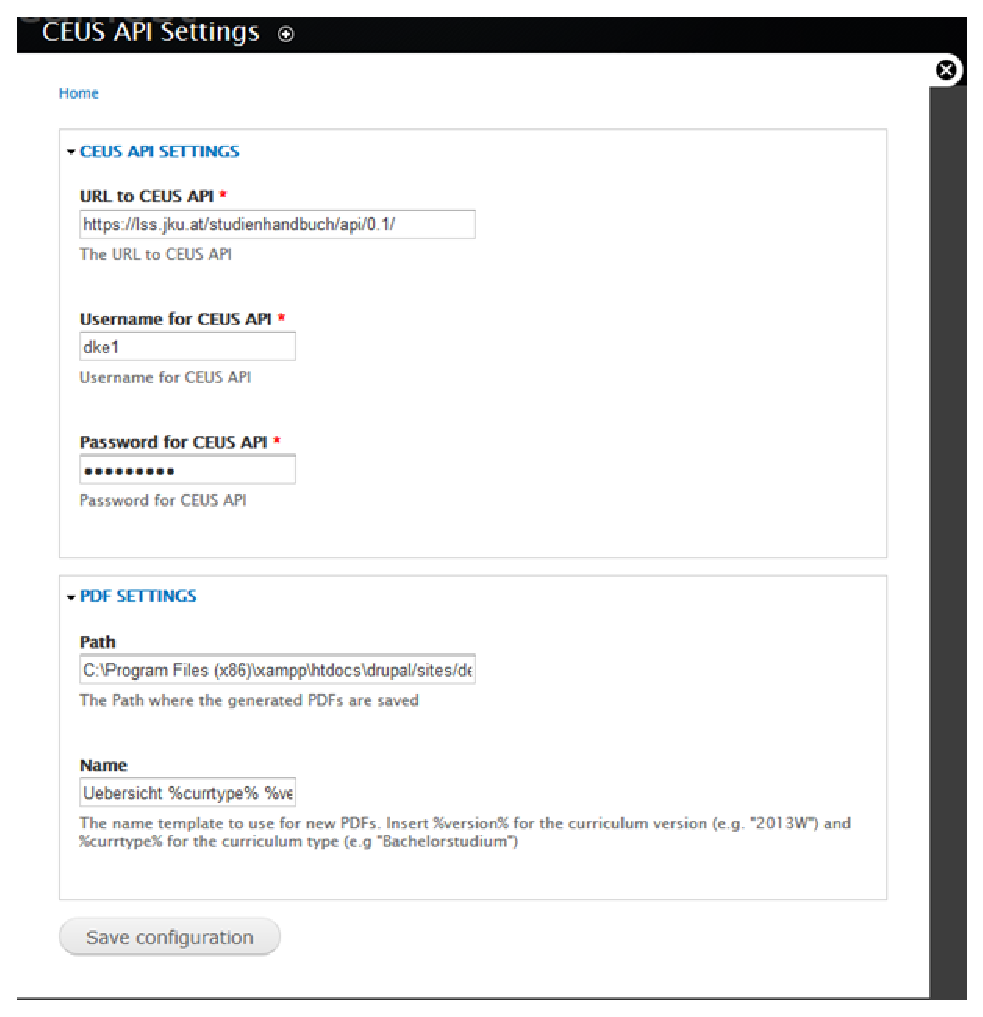
\includegraphics[width=\textwidth]{ModuleConfiguration}
\caption{Module Configuration Page}
\end{DoxyImage}


\begin{DoxyNote}{Note}
Administrator rights are needed to configure the login details
\end{DoxyNote}


 The communication between this module and CEUS occurs as shown in the included \href[pdfnewwindow]{./SequenceDiagramImport.pdf}{SequenceDiagramImport.pdf} file. 

The import from C\+E\+U\+S is performed roughly in the following steps\+:
\begin{DoxyEnumerate}
\item The {\ttfamily auth} token is requested from the C\+E\+U\+S A\+P\+I
\item All available curricula are received from the A\+P\+I
\item For each curriculum, the curriculum tree is requested from the A\+P\+I
\item For each course in the tree, the details are requested in German and English
\item During the first import, new Drupal vocabularies, vocabulary terms and content nodes are created
\item We try our best to parse the field {\ttfamily voraussetzungen} and extract relations between courses (recommended/required)
\end{DoxyEnumerate}

 This process is shown in the included \href[pdfnewwindow]{./FlowchartCEUS2Drupal.pdf}{FlowchartCEUS2Drupal.pdf} file, with the corresponding methods in \hyperlink{classceus__importer}{ceus\+\_\+importer} that perform each step.  Here is a quick textual description of the process\+:

The data import is initiated in the file \hyperlink{stukowin_8module}{stukowin.\+module}. This file first access \hyperlink{classceus__importer_a78572828d11dcdf2a498497d9001d557}{ceus\+\_\+importer\+::connect()} in the file \hyperlink{ceus__importer_8inc_8php}{ceus\+\_\+importer.\+inc.\+php} and prepares the import process. In order for this to work, the necessary settings have to be made in the configuration menu shown above. All methods for the data import are collected in the \hyperlink{ceus__importer_8inc_8php}{ceus\+\_\+importer.\+inc.\+php} file.

After this, the method \hyperlink{classceus__importer_abd2f9a9afc073169b2badcb571cc983c}{ceus\+\_\+importer\+::get\+\_\+curricula()} is called, which starts the import process. It checks if a Drupal vocabulary for the imported curricula already exists. If none are found, a new one is created. If the curricula's version numbers are different, a new vocabulary is created as well.

After getting the tree for each curriculum, the details for its courses are requested and stored.

Another noteworthy part is the method \hyperlink{classceus__importer_a04b7723caf55a2cfd4b92d02754748dc}{ceus\+\_\+importer\+::process\+\_\+relations()}. This method is responsible for parsing the field {\ttfamily voraussetzungen}, which can contain any text possible. The method examines the field in three steps\+:
\begin{DoxyEnumerate}
\item Is the field empty? If not, go to Step 2.
\item Does the field begin with \char`\"{}empfohlen\char`\"{}? If yes, it is a {\itshape recommended} relation, if not it is a {\itshape required} relation.
\item Try to find $<$li$>$ and $<$a$>$ tags and extract a course title or code from them.
\end{DoxyEnumerate}

Requirements are important mostly because they are used and shown in the \hyperlink{index_Drupal2AGG}{automatically generated graphic representation}.

All of the code for the import is contained in the \hyperlink{ceus__importer_8inc_8php}{ceus\+\_\+importer.\+inc.\+php} file.

\begin{DoxySeeAlso}{See also}
\hyperlink{group___c_e_u_s2_drupal}{C\+E\+U\+S2\+Drupal}
\end{DoxySeeAlso}
\hypertarget{index_change_management}{}\paragraph{Change Management}\label{index_change_management}
The functional requirements of this project make it necessary to periodically extract data from C\+E\+U\+S on the one hand and giving administrators and moderators the ability to overwrite data on the other hand. \begin{DoxyRemark}{Remarks}
How to overwrite course data is described in the user documentation.
\end{DoxyRemark}


 This creates the challenge of properly versioning the CMS content, which is why every import follows the rules shown in the included \href[pdfnewwindow]{./Changemanagement.pdf}{Changemanagement.pdf} file 

Every time a content node is created or updated, it gets a red {\itshape New} tag in the content overview (see image below), through which the administrator can easily see which nodes have been updated. In addition to this, the import returns a success message that tells the administrator how many nodes have been created or updated, so that one can easily tell if changes have occurred.


\begin{DoxyImage}
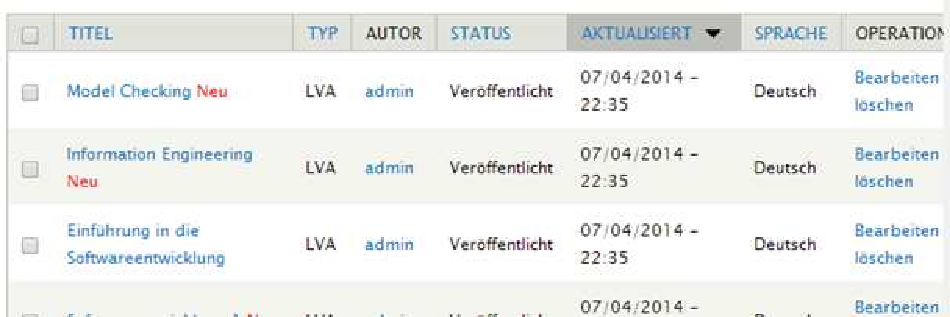
\includegraphics[width=\textwidth]{NewTag}
\caption{Red {\itshape New} Tag}
\end{DoxyImage}
\hypertarget{index_Drupal2ITSV}{}\subsubsection{Drupal2\+I\+T\+S\+V}\label{index_Drupal2ITSV}
As C\+E\+U\+S does not provide any information about fields of specialisation during the master studies and ideal courses of studies, henceforth called I\+T\+S\+V due to its German name, it was a project requirement that new curricula can be created by the administrator for such purposes.

A freely available Drupal module called Taxonomy Manager (\href{https://www.drupal.org/project/taxonomy_manager}{\tt https\+://www.\+drupal.\+org/project/taxonomy\+\_\+manager}) gives the administrator the ability to copy vocabulary terms from one vocabulary to another, which is most of the work. Unfortunately, this process cannot be simplified any further. Nevertheless, we tried to at least automate the task of creating a new vocabulary, copying all of the information over from the source curriculum and creating top-\/level terms (such as \char`\"{}1. Semester\char`\"{} etc.), tasks which will be performed every time a new I\+T\+S\+V or specialisation has to be created.

This component handles exactly that. It inserts a new menu item (at admin/settings/stukowin/taxonomy) where the administrator can select a source curriculum to base the new one on, select whether to create an I\+T\+S\+V or specialisation vocabulary, enter a name and choose how many top-\/level terms should be inserted. Once the administrator has filled out the form, the new vocabulary is automatically created and the browser is redirected to the Taxonomy Manager's \char`\"{}\+Dual View\char`\"{}, where the administrator can begin copying courses into the new vocabulary.

\begin{DoxyRemark}{Remarks}
This component does not have its own file as it does not contain a lot of code. All of its functionality is in the \hyperlink{stukowin_8module}{stukowin.\+module} file.
\end{DoxyRemark}
\begin{DoxySeeAlso}{See also}
\hyperlink{group___drupal2_i_t_s_v}{Drupal2\+I\+T\+S\+V}
\end{DoxySeeAlso}
\hypertarget{index_Drupal2PDF}{}\subsubsection{Drupal2\+P\+D\+F}\label{index_Drupal2PDF}
In order to permanently and easily archive past curricula there is the option to automatically create a course overview P\+D\+F document from the imported courses. For this component to work properly, the necessary settings have to be made in advance (see module configuration image above). The administrator is provided with a new menu (at admin/settings/stukowin/pdf) where the curriculum to be archived can be selected. Once he clicks on \char`\"{}\+Create P\+D\+F\char`\"{}, the P\+D\+F generation in \hyperlink{classoverview_p_d_f_a30ddd92aaf87bca0825c149bd3a7d43f}{overview\+P\+D\+F\+::create\+P\+D\+F()} is started. (All of the P\+D\+F generation code is contained in the \hyperlink{pdf__creator_8inc_8php}{pdf\+\_\+creator.\+inc.\+php} file)



 The PDF generation process will flow as shown in the included \href[pdfnewwindow]{./FlowchartDrupal2PDF.pdf}{FlowchartDrupal2PDF.pdf} file. 

\begin{DoxySeeAlso}{See also}
\hyperlink{group___drupal2_p_d_f}{Drupal2\+P\+D\+F}
\end{DoxySeeAlso}
\hypertarget{index_Drupal2AGG}{}\subsubsection{Drupal2\+A\+G\+G}\label{index_Drupal2AGG}
So far we have described how to import and edit curricula into Drupal. But part of the functional requirements were also being able to automatically display the curricula on the website in the form of an automatically generated graphic (A\+G\+G). This component provides the functionality for doing exactly that. Again, it can be separated into three components\+:\hypertarget{index_json}{}\paragraph{Drupal J\+S\+O\+N Interface}\label{index_json}
To make the curricula data available to clients, several J\+S\+O\+N interfaces have been implemented that make curricula publicly reachable. This is needed so that the client browser can properly display the curricula.

The following interfaces are available\+: \begin{TabularC}{4}
\hline
\rowcolor{lightgray}{\bf Name }&{\bf Path }&{\bf Input Parameter }&{\bf Description  }\\\cline{1-4}
Curriculum List &stukowin/crclmlst &\char`\"{}currtype\char`\"{} \+: Type of curriculum to get (\char`\"{}\+Bachelorstudium\char`\"{} or \char`\"{}\+Masterstudium\char`\"{})~\newline
\char`\"{}taxtypes\char`\"{} \+: Types of vocabularies to get (\char`\"{}curriculum\char`\"{}, \char`\"{}itsv\char`\"{} and/or \char`\"{}specialisation\char`\"{}) &Returns a list of all curricula currently published (weight $<$ 0), like \hyperlink{index_list}{list.\+php} \\\cline{1-4}
Curriculum Tree &stukowin/crclm &Vocabulary id of the curriculum to get &Returns the curriculum tree of one curriculum, containing all courses and their details \\\cline{1-4}
Single course &stukowin/lva &Node id of the course to get &Returns the details of a single course \\\cline{1-4}
\end{TabularC}
All of these interfaces are defined in the \hyperlink{stukowin_8module}{stukowin.\+module} file.\hypertarget{index_plugin}{}\paragraph{C\+K\+Editor Plug-\/in}\label{index_plugin}
As the dynamic display of curricula in the browser requires a strict H\+T\+M\+L document structure, we refrained from letting the administrator insert the code himself wherever a curriculum display was needed and instead implemented a plug-\/in for the C\+K\+Editor (\href{https://www.drupal.org/project/ckeditor}{\tt https\+://www.\+drupal.\+org/project/ckeditor}) which inserts the code automatically on the click of a button. The plug-\/in is registered with drupal in the \hyperlink{group___drupal2_a_g_g_gae3c906d1ab9c3d8ed245d58c1ebf2a4a}{stukowin\+\_\+ckeditor\+\_\+plugin()} method. It is then defined in the \hyperlink{plugin_8js}{plugin.\+js} file and the dialog for inserting a curriculum view is defined in the \hyperlink{stukowin__curriculum_8js}{stukowin\+\_\+curriculum.\+js} file.

\begin{DoxyNote}{Note}
In order for this plug-\/in to work properly, some settings have to be made in the C\+K\+Editor. This is described in the operator manual.
\end{DoxyNote}
\hypertarget{index_graph}{}\paragraph{Graph.\+js}\label{index_graph}
The main task of displaying the curricula in the client's browser is performed by this file. It fetches the data from the J\+S\+O\+N interfaces described \hyperlink{index_json}{above} and creates the D\+O\+M elements in the browser. It also registers click handlers for things such as expanding/reducing a course, showing prerequisites and selecting a different curriculum. \begin{DoxyNote}{Note}
The display layout is configured in the curriculum\+\_\+stlye.\+css file (not included in this documentation)
\end{DoxyNote}
As an example, the output could look like this\+:


\begin{DoxyImage}
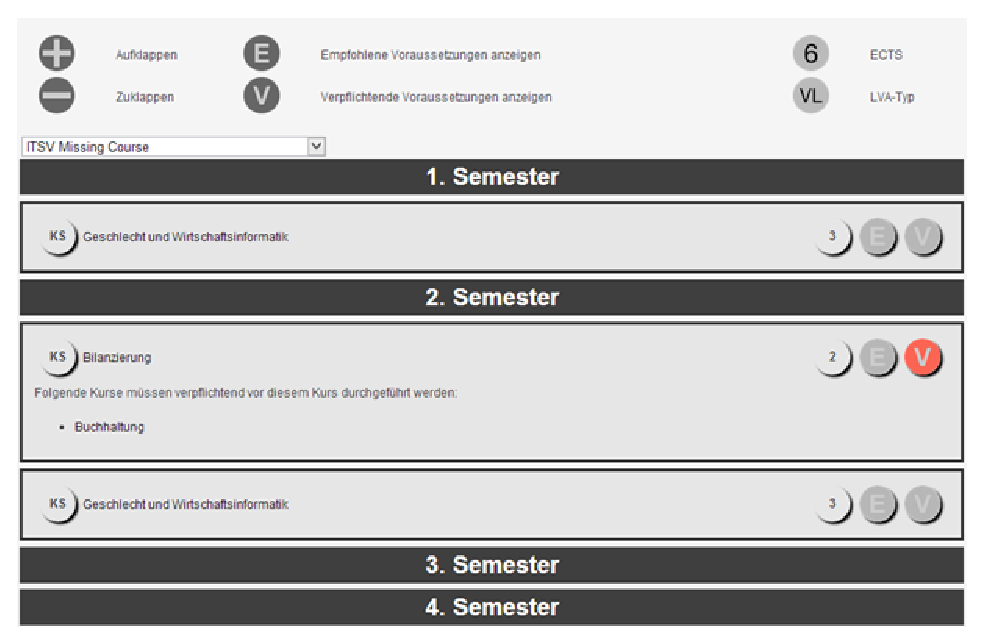
\includegraphics[width=\textwidth]{Drupal2AGG}
\caption{Graphical Representation}
\end{DoxyImage}


\begin{DoxySeeAlso}{See also}
\hyperlink{group___drupal2_a_g_g}{Drupal2\+A\+G\+G}
\end{DoxySeeAlso}
\hypertarget{index_Other}{}\subsubsection{Other}\label{index_Other}
All of the components described above need to work together somehow and at the same time be accessible to Drupal itself. For this reason there are several methods and files to ensure a smooth cooperation, some of which are worth mentioning explicitly\+:
\begin{DoxyItemize}
\item The \hyperlink{classcontent__manager}{content\+\_\+manager} class is responsible for accessing the imported curricula data
\item The \hyperlink{stukowin_8install}{stukowin.\+install} file is responsible for installing and uninstalling the module and all the data structures that come with it
\item The \hyperlink{group___stukowin___module_ga59cfbad113b7aa2d10f0b204a5f7ba0d}{stukowin\+\_\+menu()} function sets up all the callback U\+R\+Ls
\item The \hyperlink{group___stukowin___module_ga55d453d5b6f8ae4e643308d8814e67a5}{stukowin\+\_\+admin()} function is responsible for the configuration menu
\item The stukowin.\+info file contains all meta information about the module
\end{DoxyItemize}\hypertarget{index_Development}{}\subsection{Development}\label{index_Development}
\hypertarget{index_Authors}{}\subsubsection{Authors}\label{index_Authors}
\begin{DoxyNote}{Note}
Every file, class, method and member is documented with an {\ttfamily @author} tag. The person tagged as {\ttfamily @author} (thus being shown as the author) is the main/initial author of that file, class, method or member. 

All other authors, (people that have helped during initial development, fixed bugs or made changes) are tagged with the {\ttfamily @author{\bfseries s} }(plural) tag, thus being shown under Author{\bfseries s(plural)}. 

If a file, class, method or member has been authored by multiple people equally, all of them are tagged with the {\ttfamily @author{\bfseries s} tag} and there is no {\ttfamily @author}. 

If you have any questions regarding the system, feel free to contact the respective author.
\end{DoxyNote}
The following list shows an overview of every person that has participated in writing this module, with a quick summary of what they have mostly contributed to\+:
\begin{DoxyItemize}
\item {\bfseries Jakob Strasser} -\/ \href{mailto:jakob.strasser@telenet.be}{\tt jakob.\+strasser@telenet.\+be} ~\newline
Main author of the \hyperlink{index_CEUS2Drupal}{P\+D\+F generation component} and the \hyperlink{graph_8js}{graph.\+js} file. Participating author in most files/components. 


\item {\bfseries Konstantinos Dafalias} -\/ \href{mailto:kdafalias@gmail.com}{\tt kdafalias@gmail.\+com} ~\newline
Mostly responsible for the \hyperlink{index_CEUS2Drupal}{C\+E\+U\+S import} and the \hyperlink{group___stukowin___module}{Module Core} 


\item {\bfseries Werner Breuer} -\/ \href{mailto:bluescreenwerner@gmail.com}{\tt bluescreenwerner@gmail.\+com} ~\newline
Co-\/author of the \hyperlink{index_plugin}{C\+K\+Editor Plug-\/in} and the \hyperlink{index_Drupal2AGG}{Drupal2\+A\+G\+G} component in general, as well as the \hyperlink{index_Drupal2ITSV}{Drupal2\+I\+T\+S\+V} component. Participated in a lot of debugging. 


\item {\bfseries Markus Gutmayer} -\/ \href{mailto:m.gutmayer@gmail.com}{\tt m.\+gutmayer@gmail.\+com} ~\newline
Co-\/author of the \hyperlink{index_plugin}{C\+K\+Editor Plug-\/in} and the \hyperlink{index_Drupal2AGG}{Drupal2\+A\+G\+G} component in general, as well as the \hyperlink{index_Drupal2ITSV}{Drupal2\+I\+T\+S\+V} component. Participated in a lot of debugging. 


\item {\bfseries Fabian Puehringer} -\/ \href{mailto:f.puehringer@24speed.at}{\tt f.\+puehringer@24speed.\+at} ~\newline
Assistance with \hyperlink{index_Drupal2PDF}{Drupal2\+P\+D\+F} and \hyperlink{index_Drupal2AGG}{Drupal2\+A\+G\+G} 


\item {\bfseries Manuel Muehlburger} -\/ \href{mailto:Hansbert92@googlemail.com}{\tt Hansbert92@googlemail.\+com} ~\newline
Layout and design for the \hyperlink{index_Drupal2AGG}{Drupal2\+A\+G\+G} component (mainly the \hyperlink{index_graph}{Graph.\+js})
\end{DoxyItemize}\hypertarget{index_versionnumbers}{}\subsubsection{Version Numbers}\label{index_versionnumbers}
Every file and class has a version number, composed of four parts\+: {\itshape major.\+minor.\+revision} {\itshape date} 
\begin{DoxyItemize}
\item {\itshape Major} signifies a major release, such as the initial release
\item {\itshape Minor} signifies the addition of a new feature
\item {\itshape Revision} signifies a bug fix or something similarly small
\item {\itshape Date} shows when the last change was made to the source code (in the format \char`\"{}\+Y\+Y\+Y\+Y-\/\+M\+M-\/\+D\+D\char`\"{})
\end{DoxyItemize}\hypertarget{index_versioncontrol}{}\subsubsection{Version Control}\label{index_versioncontrol}
When the project started, there were two groups, each of which used a different version control system. Group 1 used S\+V\+N on \href{http://cloudforge.com}{\tt http\+://cloudforge.\+com} while group 2 used \href{http://bitbucket.org}{\tt http\+://bitbucket.\+org}. When the two groups were merged, the S\+V\+N repository was dropped. Due to privilege problems with bitbucket, it was decided to move the entire repository to \href{http://github.com}{\tt http\+://github.\+com}, as everyone had access there. At the time writing this documentation, the repository is available at \href{http://github.com/TheJake123/DrupalModul}{\tt http\+://github.\+com/\+The\+Jake123/\+Drupal\+Modul}.

As the repository is open source, the commit, issue and change history can be publicly viewed. Additionally, every file, class, method and member has been documented with a {\ttfamily @since} tag with the following format\+: \char`\"{}\+Commit $<$hash$>$ on Y\+Y\+Y\+Y-\/\+M\+M-\/\+D\+D\char`\"{}, so that it is easily visible when a file, class, method or member has been added.\hypertarget{index_Included}{}\subsection{Included Libraries/\+Files}\label{index_Included}
For the P\+D\+F generation, the free and open source library \href{http://www.tcpdf.org/}{\tt T\+C\+P\+D\+F} is used and included in the project.

For parsing course relationships, the \href{http://simplehtmldom.sourceforge.net/}{\tt simple\+\_\+html\+\_\+dom.\+php} file is used 